Large Language Models (LLMs) are data-driven AI that process and generate human-like text. Built on transformer architectures and trained on vast datasets, LLMs like GPT, BERT, Claude and LLaMA can perform various language tasks with remarkable fluency. LLM-based agents extend these capabilities by integrating them into systems that can tackle complex real-world problems.
This chapter explores advanced techniques for harnessing LLMs' reasoning abilities through prompt engineering and introduces concepts for developing problem-solving agents using LLMs as a core.

\section{LLMs: Designing Effective Prompts}
\label{sec:effectiveprompts}
This section analyzes techniques for designing effective prompts, ranging from basic principles to advanced concepts like retrieval-augmented generation and automatic prompt engineering. 

\subsection{LLM-setting}
When working with LLMs via an API, adjusting specific parameters can significantly influence the model's outputs, and understanding these settings is crucial for optimizing results. 

The \textbf{Temperature} parameter is used in the sampling process of generating text, controlling the randomness of the output. Mathematically, it modifies the probability distribution over the next token to be selected. Given a probability distribution \( P(x_i) \) over the possible next tokens \( x_i \), the temperature \( T \) modifies this distribution as follows: \[
P'(x_i) = \frac{P(x_i)^{1/T}}{\sum_j P(x_j)^{1/T}}
\]
where \( P(x_i) \) is the original probability of token \( x_i \), \( P'(x_i) \) is the adjusted probability after applying the temperature and \( T \) is the temperature value.
It follows that when \( T < 1 \) the distribution sharpens while when \( T > 1 \) the distribution flattens, making the probabilities more uniform.

The \textbf{Top P (Nucleus Sampling)} works with temperature to control the diversity of responses. Top P determines the probability mass of tokens considered for the next output. A low Top P value (e.g., 0.1) restricts the model to the most likely tokens, yielding more precise and factual responses. Higher Top P values allow for a broader range of token choices, increasing output diversity.

The \textbf{Max Length} limits the number of tokens the model generates in response to a prompt. This is useful for controlling the length of responses and preventing the generation of overly long or off-topic content, which also helps manage API costs.

The \textbf{Frequency Penalty} setting discourages the repetition of tokens by applying a penalty proportional to how often a token has already appeared. A higher frequency penalty makes the model less likely to repeat words, which is beneficial for generating more varied text.

The \textbf{Presence Penalty}, similar to the frequency penalty, uniformly penalizes all repeated tokens, regardless of how many times they have appeared. This setting is useful for preventing the model from reiterating phrases or concepts excessively, thus encouraging more diverse output.

Generally, it's recommended to adjust either temperature or Top P, and either frequency or presence penalty, rather than altering both pairs simultaneously. This targeted tweaking helps in fine-tuning the model's behaviour for specific tasks.
Experimentation with these settings is key, as the optimal configuration can vary depending on the version of the LLM and the specific use case.

\subsection{Techniques To Design Effective Prompts}
\label{sec:prompts}
LLMs are trained to maximize the next token in a sequence of text, given the preceding context. The effectiveness of an LLM in generating coherent, contextually relevant, and accurate responses depends on its ability to model complex linguistic patterns. This is achieved through the attention mechanism, which allows the model to weigh the importance of different tokens and update based on previous text. Designing effective prompts is therefore an essential skill when interacting with generative LLMs. Several techniques can be employed: the quality and relevance of the model's output are highly sensitive to the prompt design.

In this subsection, we will explore various strategies that can be employed to optimize prompt design.

\paragraph{Clarity and Specificity}

One of the most crucial aspects of crafting effective prompts is ensuring clarity and specificity. Ambiguity in a prompt often leads to ambiguous or irrelevant outputs, as the model attempts to interpret the prompt in multiple ways. Therefore, it is essential to use clear and concise language, avoiding unnecessary jargon unless it is contextually appropriate and well-understood by the model.

When designing a prompt, specificity is equally important. A prompt that is too broad may result in a generalized response, lacking the depth or focus needed for a particular task. 

\paragraph{Contextual Framing}

Providing context is another powerful technique for prompt design. Contextual framing helps the model to understand the background and nuances of the task at hand, enabling it to generate more accurate and relevant responses. This can be achieved by including background information, setting the scene, or specifying the perspective from which the model should respond. This technique is also named profiling.

For example, suppose the goal is to generate a narrative from the perspective of a historical figure. The prompt might be: "Imagine you are Leonardo da Vinci, and you are writing a letter to a fellow artist explaining your latest invention. Describe the invention and your inspiration behind it." This prompt specifies the task and immerses the model in a particular context, guiding it to produce a more coherent and contextually appropriate response.

\paragraph{Incorporating Examples}

Another effective technique is the use of examples within the prompt. Providing examples helps to set clear expectations for the model, illustrating the format, style, or level of detail required in the response. This is particularly useful when the task involves generating creative content, solving problems, or following specific guidelines. Based on the number of examples provided, we name it zero-shot (no examples), few-shot and many-shot learning. 

For example, if the task is to generate a poem in the style of a famous poet, the prompt could include an excerpt from one of the poet's works as an example. The prompt might be structured as follows: "Write a poem in the style of William Wordsworth. For reference, here is an excerpt from 'I Wandered Lonely as a Cloud': [insert excerpt]. Use similar language and themes in your poem."

In-context learning methods may effectively tweak the model output to solve the task but sometimes results are controversial. More on this in the in-context learning section \ref{in-context-learning}

\paragraph{Defining Constraints}

Defining constraints is a technique that can help to narrow the focus of the model's response, ensuring it remains relevant to the task at hand. Constraints can be related to word count, format, tone, or specific content requirements. By clearly defining these constraints within the prompt, the model is better equipped to produce a response that aligns with the user's expectations.

For example, if the task requires a succinct summary, the prompt might include a constraint such as: "Summarize the main arguments of the article in no more than 150 words."

\paragraph{Balancing Specificity with Flexibility}

While specificity is crucial, it is also important to balance it with flexibility, depending on the task. Overly rigid prompts can stifle creativity or limit the scope of the model's response. Therefore, in some cases, allowing for a degree of flexibility within the prompt can be beneficial.

For example, instead of asking the model to "List three reasons why climate change is a pressing issue," a more flexible prompt might be, "Discuss why climate change is considered a critical global challenge, providing examples where relevant." This allows the model to explore the topic more freely while still adhering to the prompt's overall objective.

\paragraph{Iterative Refinement: Testing and Feedback}

Effective prompt design is often an iterative process. The initial prompt might not always yield the desired output, necessitating revisions and refinements. Iterative refinement involves analyzing the output generated by the model in response to a given prompt and then tweaking the prompt to address any shortcomings or gaps in the response.

Testing the prompts and gathering feedback is an essential part of the prompt design process. By testing prompts with different variations and obtaining feedback on the generated outputs, designers can identify strengths and weaknesses in their prompt design. This process often reveals insights into how the model interprets different phrasings or instructions, allowing for further refinements.

Feedback can be gathered either through user testing or by analyzing the responses generated by the model. This iterative cycle of testing and feedback ensures that prompts are continuously improved, leading to more effective and reliable interactions with the AI.

In conclusion, designing effective prompts involves a careful balance of clarity, specificity, context, and flexibility. By employing these techniques and engaging in iterative refinement, prompt designers can significantly enhance the quality and relevance of the model's output, ensuring it meets the desired objectives.

\subsection{Structuring Reasoning}
Prompt techniques are a way to guide outputs/reasoning to improve the LLMs' performance and reliability. Let's show the most effective ones:
\begin{itemize}
    \item The \textbf{Chain of Thought} (CoT \cite{wei2023chainofthought}) prompting technique aims to generate more accurate and detailed responses by breaking down the problem or question into smaller, sequential logical steps. This technique helps the AI model systematically reason through the problem, rather than jumping directly to an answer.
    
    \item The \textbf{Tree of Thought} (ToT \cite{yao2023tree}) consists of exploring multiple potential solutions simultaneously, akin to branching in a tree structure.
    
    \item The \textbf{Self-consistency} \cite{wang2023selfconsistency} prompting consists of generating multiple answers to a single prompt and then consolidating these answers to find a consistent, common solution. This approach helps to mitigate the variability and potential errors in individual responses by leveraging the consensus among multiple outputs. 

    \item A \textbf{Meta-prompting} \cite{zhang2024metapromptingaisystems} is an example-agnostic structured prompt designed to capture the reasoning structure of a specific category of tasks. It provides a scaffold that outlines the general approach to a problem, enabling LLMs to fill in specific details as needed. This approach allows for more efficient and targeted use of LLM capabilities by focusing on the "how" of problem-solving rather than the "what".
\end{itemize}
To exemplify, we experimented with an arithmetic-based task: the game 24~\ref{chap:appendix_a}.

\subsection{In-Context Learning and Fine-Tuning}
\label{in-context-learning}
In the realm of machine learning, particularly within the domain of natural language processing (NLP), in-context learning (ICL) and fine-tuning represent two pivotal paradigms for adapting models to new tasks. In-context learning leverages LLMs to perform tasks by utilizing examples provided directly in the input context, without modifying the model's parameters. Fine-tuning, in contrast, involves training a pre-existing model on new data to optimize its performance on specific tasks.

\paragraph{In-Context Learning}
The fundamental idea behind ICL is that LLMs can make predictions or generate responses based on examples embedded within the input context, without any explicit parameter updates. This process is akin to how humans learn by analogy—by drawing parallels between provided examples and new situations.

This method comes with various advantages:
\begin{itemize}
    \item Flexibility: ICL allows for rapid adaptation to new tasks without retraining;
    \item Data Efficiency: ICL is particularly useful in scenarios with limited data, as it can perform reasonably well with just a few examples provided in the context.
    \item Interpretability: Since the demonstrations are written in natural language, ICL offers an interpretable interface that allows for easy integration of human knowledge into the model.
\end{itemize}

However, the performance of ICL is sensitive to several factors, including the quality of the prompt, the selection and order of demonstration examples, and the specific settings of the LLM \cite{dong2024surveyincontextlearning}. Despite these sensitivities, ICL has been shown to perform well across a wide range of tasks, including mathematical reasoning \cite{yang2023leandojotheoremprovingretrievalaugmented}.

\paragraph{Fine Tuning} This approach involves adapting a pre-trained model to a new task by further training it on task-specific data. Fine-tuning allows the model to optimize its parameters for the nuances of the new task, often resulting in superior performance compared to a general-purpose model.

The process generally involves freezing some layers of the pre-trained model and updating others, a technique that preserves the general knowledge acquired during the initial training while adapting to the new task \cite{wang2023egeriaefficientdnntraining}.

Another method to fine-tune a general model while avoiding a decline in its overall performance is to use KL divergence as a penalty during the update process. A virtuous example is the Reinforcement Learning from Human Feedback (RLHF) \cite{kaufmann2024surveyreinforcementlearninghuman}, where the KL divergence is used as a regularization technique to maintain the balance between a pre-trained model and its fine-tuned version.

Fine-tuning has several key strengths:
\begin{itemize}
    \item Specialization: It produces highly specialized models that are finely tuned to excel at specific tasks, which is particularly beneficial in applications requiring high accuracy.
    \item Robustness: Fine-tuned models tend to perform more reliably on the tasks they are optimized for, especially when compared to the more generalist ICL approach.
\end{itemize}


However, fine-tuning also has its limitations:
\begin{itemize}
    \item Resource Intensive: Fine-tuning requires substantial computational resources and time, particularly for large models and datasets.
    \item Maintenance Complexity: Managing multiple fine-tuned models for different tasks can be complex and resource-intensive, especially as the number of tasks grows.
\end{itemize}

\subsection{Retrieval-Augmented Generation for LLMs}
Retrieval-augmented generation (RAG) systems represent a significant evolution in natural language processing (NLP), particularly in enhancing the capabilities of large language models (LLMs). These systems integrate external knowledge sources into LLMs, addressing challenges like hallucinations, outdated information, and untraceable reasoning processes, which are inherent in models that rely solely on pre-existing data. RAG systems are particularly valuable in knowledge-intensive tasks, enabling continuous updates and the integration of domain-specific information \cite{gao2024retrievalaugmentedgenerationlargelanguage}.

\subsubsection{RAG Framework Components}
\label{sec:RAG}
A RAG system typically consists of three primary components: retrieval, generation, and augmentation. These components work together to enable the LLM to generate more accurate and contextually relevant responses.

\paragraph{Retrieval}

The retrieval component is responsible for sourcing relevant information from external databases or knowledge repositories. The process begins with indexing documents, which are often divided into smaller chunks to improve the efficiency of retrieval. These chunks are encoded into vector representations using embedding models and stored in a vector database. When a user query is received, it is similarly encoded, and the system retrieves the top k chunks that are most semantically similar to the query.

Indexing strategies vary, with some systems employing a fixed token length for chunks, while others use more sophisticated methods like sliding windows or recursive splits to maintain context continuity. Additionally, attaching metadata (such as timestamps or file names) to chunks can enhance retrieval by allowing more precise filtering.

\paragraph{Generation}

After retrieval, the selected document chunks are combined with the original query to form a prompt for the LLM. The model generates a response based on this augmented prompt. 
To overcome hallucinations, RAG systems may employ fine-tuning techniques that adjust the model's behaviour based on specific data or task requirements. Additionally, strategies like context compression or re-ranking of retrieved information can be used to improve the relevance and coherence of the generated response.

\paragraph{Augmentation}

Augmentation involves enhancing the retrieved information before it is fed into the LLM for generation. This can include iterative retrieval processes, where the system continuously refines its search based on the generated text, or adaptive retrieval, where the LLM decides when additional information is needed.

Advanced RAG systems have introduced modular architectures that allow for greater flexibility in handling complex queries. For instance, some systems incorporate a "memory" module that stores previously retrieved information for reuse, or a "predict" module that generates context directly from the LLM, reducing the need for external retrieval.

\subsubsection{RAG Paradigms}

The development of RAG systems has progressed through several stages:
\begin{itemize}
    \item Naive RAG: This initial approach follows a straightforward retrieval-generation process. It is effective but limited by challenges in retrieval accuracy and the potential for generating irrelevant or hallucinated content.

    \item Advanced RAG: Building on the naive approach, advanced RAG introduces optimization techniques in both retrieval and generation. For example, it may use fine-grained segmentation in indexing or employ query expansion techniques to improve retrieval relevance.

    \item Modular RAG: The most flexible and adaptable paradigm, modular RAG systems can incorporate various specialized modules to enhance retrieval and generation. This architecture supports more complex retrieval processes, such as iterative or adaptive retrieval, and allows dynamic integration with other technologies like reinforcement learning.
\end{itemize}
% TODO ADD CITATIONS


\subsection{Automatic Prompt Engineering}
\label{sec:autoprompts}
The evolution of LLMs has brought about a renewed focus on prompt engineering. This technique focuses on crafting effective queries for LLMs to maximize task performance. Several approaches are being explored, including Prompt-OIRL, OPRO, AutoPrompt and Prefix Tuning, each bringing unique methodologies and improvements to the field.

\subsubsection{Offline Inverse Reinforcement Learning for Query-Dependent Prompts}

Prompt-OIRL \cite{sun2024querydependentpromptevaluationoptimization} represents an innovative approach to prompt engineering by integrating concepts from offline inverse reinforcement learning (IRL). In traditional reinforcement learning (RL), the goal is to learn optimal policies based on rewards observed during the agent's interactions with an environment. However, inverse reinforcement learning takes a different path, focusing on deducing the underlying reward function that explains the observed behaviours of an expert.

Prompt-OIRL proposes to generate query-dependent prompts by leveraging IRL principles in an offline setting. The idea here is to learn a reward function that explains the relationship between user queries and effective prompts by analyzing historical data. Once the model learns this reward function, it can generate optimized prompts for new queries without requiring additional online interactions, making the process more efficient.

The key advantage of Prompt-OIRL lies in its adaptability. Since it uses an offline dataset of expert query-prompt pairs, it can generalize well to unseen queries while maintaining high performance. This makes it a powerful tool in domains where direct online interactions are costly or time-consuming. For instance, in a customer service application, Prompt-OIRL could generate tailored prompts based on user input, improving response relevance and efficiency without needing real-time feedback loops.

\subsubsection{OPRO: Optimizing Prompts with LLMs}

The OPRO (Optimizing Prompts) technique takes a different approach to automatic prompt engineering by directly leveraging the capabilities of large language models (LLMs) to refine and optimize prompts. One notable example from this method is the "Take a deep breath" prompt modification, which significantly enhances the performance of LLMs on complex tasks such as math problem-solving.

In traditional prompt engineering, the choice of wording can profoundly influence model outputs. OPRO introduces the idea that LLMs themselves can be used to iteratively refine prompts by testing slight modifications and evaluating the impact on task performance.

This technique highlights the potential for automatic prompt optimization through a self-supervised feedback loop, where the LLM refines its own input prompts based on performance. It is an efficient way to unlock latent capabilities within the model, without requiring extensive external datasets or human supervision.

\subsubsection{AutoPrompt: Gradient-Guided Prompt Creation}

AutoPrompt \cite{shin2020autopromptelicitingknowledgelanguage} is another cutting-edge approach to automatic prompt generation that introduces the concept of using gradient-guided search to automatically create prompts for diverse tasks. Unlike manual prompt crafting, AutoPrompt treats the process of prompt creation as an optimization problem, where the goal is to discover the prompt that maximizes model performance on a given task.

The core idea behind AutoPrompt is to use gradients from the model's loss function to guide the search for optimal prompts. By backpropagating through the model, AutoPrompt can iteratively adjust the prompt tokens to improve task performance, effectively tuning the input in a way that maximizes accuracy or other performance metrics. This approach is particularly well-suited for tasks where hand-crafted prompts may be suboptimal or infeasible due to the complexity of the task.

\subsubsection{Prefix Tuning: A Lightweight Alternative to Fine-Tuning}

While traditional fine-tuning of LLMs involves updating all or most of the model parameters, Prefix Tuning \cite{li2021prefixtuningoptimizingcontinuousprompts} offers a more lightweight and efficient alternative. Instead of modifying the entire model, Prefix Tuning introduces the concept of prepending a trainable continuous prefix to the input, which serves as a prompt that steers the model’s outputs for natural language generation (NLG) tasks.

Prefix Tuning is particularly useful in scenarios where computational resources are limited, or when it is impractical to fine-tune the entire model for each specific task. The trainable prefix acts as a form of learned prompt that influences the model’s outputs without requiring extensive parameter updates.

In contrast to standard prompt engineering, which typically involves hand-crafting or automatically generating discrete prompts, Prefix Tuning allows for continuous, differentiable prompts that can be optimized through gradient descent. This opens up new possibilities for fine-tuning LLMs more efficiently, particularly in scenarios involving few-shot or zero-shot learning, where minimal task-specific data is available.

\section{LLM-Based Agents}
\label{sec:llmbasedagent}
In the context of Large Language Models (LLMs), agents leverage natural language understanding and generation capabilities to interact with users and other systems. These LLM-based agents can perform complex language tasks, such as text summarization, translation, and conversational dialogue, by integrating the inherent strengths of LLMs with the autonomous characteristics of agents. This combination allows for the creation of sophisticated systems capable of handling a wide range of applications in natural language processing and beyond.

Understanding the foundational concepts of agents sets the stage for exploring the unified framework for designing LLM-based autonomous agents, as discussed in the subsequent sections.

\subsection{Agency: a General Overview}

The term "agent" refers to a computational entity that acts on behalf of a user or another program, exhibiting a certain level of autonomy. In this section we first consider the general properties of the agency, then we delve into an LLM-related framework and finally, we discuss whether scaffolded LLMs can become a general-purpose technology.


\subsubsection{Defining Characteristics of Agents}
The concept of an agent is broad and encompasses a variety of definitions and functionalities, which are useful to understand before delving into the specifics of LLM-based agents.
An agent is generally characterized by its ability to operate autonomously, make decisions, and perform actions without direct human intervention. It's defined by the ability to perceive its environment through sensors and act upon that environment through actuators. Autonomy allows agents to manage tasks efficiently and respond to changes in their environment.

To clarify the concept further, agents typically exhibit several key properties:

\begin{itemize}
    \item \textbf{Autonomy}: Agents can operate independently, using their internal mechanisms to decide on actions based on their objectives and perceptions.
    \item \textbf{Reactivity}: They perceive their environment through sensors or data inputs and react to changes promptly and contextually.
    \item \textbf{Proactiveness}: Agents can take the initiative, exhibiting goal-directed behaviour to achieve specific objectives rather than merely reacting to external stimuli.
    \item \textbf{Adaptation}: Advanced agents can learn from their experiences, allowing them to adapt their behaviour to improve performance over time.
    \item \textbf{Social ability}: Many agents are designed to interact with other agents or humans, using communication protocols to coordinate actions and share information effectively.
\end{itemize}

% \subsubsection{Types of Agents}

% To accommodate the wide range of tasks and environments in which agents operate, various types of agents have been developed, each with specific capabilities:

% \textbf{Reflex Agents}: These agents function based on current perceptions, with their actions determined by condition-action rules. They do not consider historical data, making them suitable for straightforward tasks in predictable environments. A simple reflex agent might be a thermostat. It detects the current temperature and adjusts the heating or cooling system to maintain a set temperature, based on predefined rules.

% \textbf{Utility-Based Agents}: These agents aim to maximize a utility function, representing a performance measure. Utility-based agents can make complex decisions that optimize their overall effectiveness by balancing multiple goals and preferences. The field of reinforcement learning seeks to develop utility-based agents capable of thriving in a specific but of any kind environment. To achieve this, agents must overcome a variety of challenges, including model-free scenarios, partial observability, discrete control tasks, high-dimensional state or action spaces, and sparse rewards. In Figure \ref{fig:utility-based} we highlight the evolution of the reinforcement-learning approach to tackle games.

% \begin{figure}
%     \centering
%     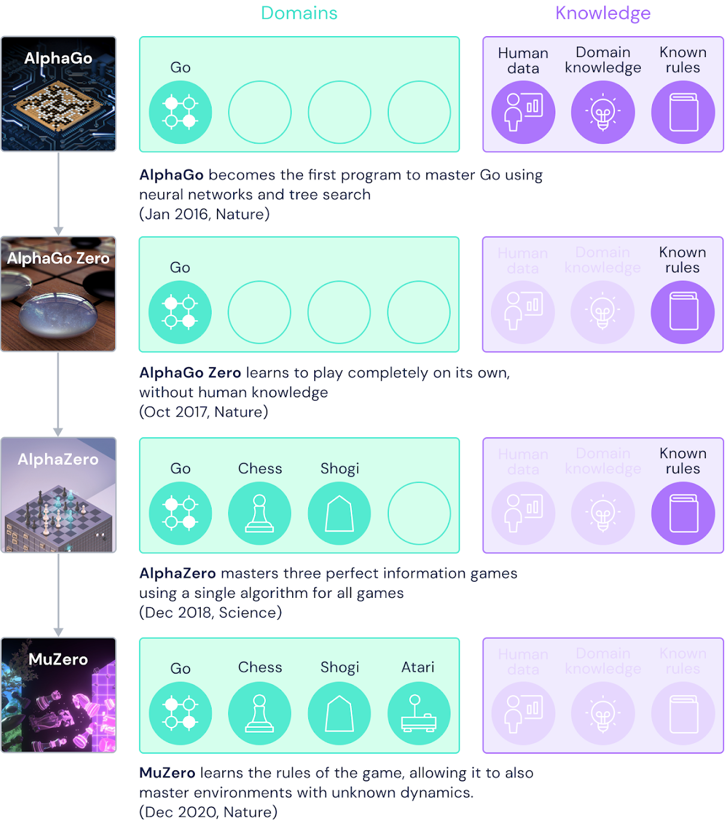
\includegraphics[width=0.9\linewidth]{Figures/agents-utilitybased.png}
%     \caption{The evolution of utility-based agents in games.}
%     \label{fig:utility-based}
% \end{figure}

% \textbf{Learning Agents}: These agents improve their performance over time through learning mechanisms. They adapt to new situations based on past experiences, making them highly versatile and capable of handling dynamic environments. A modern LLM-based example of a learning agent is given by Voyager [\cite{wang2023voyageropenendedembodiedagent}]: it's a lifelong learning agent in Minecraft that continuously explores the world, acquires diverse skills and makes novel discoveries without human intervention. It consists of three
% key components: 
% \begin{itemize}
%     \item an automatic curriculum that maximizes exploration;
%     \item an ever-growing skill library of executable code for storing and retrieving complex behaviours;
%     \item an iterative prompting mechanism that incorporates environment feedback, execution errors, and self-verification for program improvement.
% \end{itemize}
    
% The necessity of these different types lies in the varied demands of real-world applications. From simple automation tasks to complex problem-solving scenarios, each type of agent offers strengths and capabilities suited to specific needs. 

\subsubsection{Agent Scopes}
The functionality of agents spans a wide spectrum, reflecting their versatility and applicability in numerous fields:

\textbf{Task Automation}: Agents can automate repetitive and mundane tasks, freeing up human resources for more complex activities. This capability is widely used in industries ranging from manufacturing to customer service.

\textbf{Information Retrieval}: Agents can search for and aggregate information from various sources, providing users with relevant and concise data. This functionality is crucial in fields such as research and business intelligence.

\textbf{Decision Support}: By analyzing data and modelling potential outcomes, agents can assist in making informed decisions. This is particularly valuable in areas like finance, healthcare, and strategic planning.

\textbf{Human-Computer Interaction}: Agents enhance user interfaces by providing natural language processing, personalized recommendations, and interactive support. This improves user experience and accessibility.

\textbf{Robotic Control}: In robotics, agents can control physical systems, enabling autonomous navigation, manipulation, and interaction with the environment. This application is essential in fields such as space exploration, military operations, and service robotics.


\subsection{LLM-Based Agents: a General Framework}\label{agent modules}
The unified framework for designing LLM-based autonomous agents \cite{Wang_2024} consists of four main modules: profiling, memory, planning, and action. These modules work together to create a comprehensive system for autonomous agent functionality\footnote{Keep in mind that, for current LLMs, inputs must be reduced in an ad-hoc (textual) prompt at each interaction}.

\begin{itemize}
    \item \textbf{Profiling Module}: This module defines the agent's role and goal. It is crucial to establish the purpose and objectives that the autonomous agent is designed to achieve. This is achieved by crafting \textit{ad-hoc} prompts; see Sections \ref{sec:prompts} and \ref{sec:autoprompts} for details. 

    \item \textbf{Memory Module}: This module allows the LLM to read, write and access the stored information. The memory module can be conceptualized in different forms:
    \begin{itemize}
        \item \textbf{Unified Memory}: In this approach, information is written directly into the next prompts, ensuring that all relevant data is carried forward seamlessly.
        \item \textbf{Long-Term Memory}: Here, information is stored in an external support and can be recalled when needed. This allows the agent to retain important details over extended periods and retrieve specifics from huge data through a RAG method \ref{sec:RAG}.
        \item \textbf{Hybrid Memory}: This is a combination of both unified and long-term memory, leveraging the advantages of both methods to create a more versatile memory system.
    \end{itemize}

    \item \textbf{Planning Module}: This module enables the agent to plan actions based on its goals and feedback from the environment. The agent needs to develop strategies and sequences of actions that align with its objectives and adapt to changes in its surroundings. Due to the LLM's limited capability, the planning module is usually external, obtained by pipelining prompts.

    \item \textbf{Action Module}: This module translates the agent's outputs into specific outcomes through tools and APIs. It is responsible for executing the planned actions and interacting with the external environment to achieve the desired results.
\end{itemize}

Each module can be implemented with different strategies and formats, mostly illustrated in Figure \ref{fig: agent}.
\begin{figure}
    \centering
    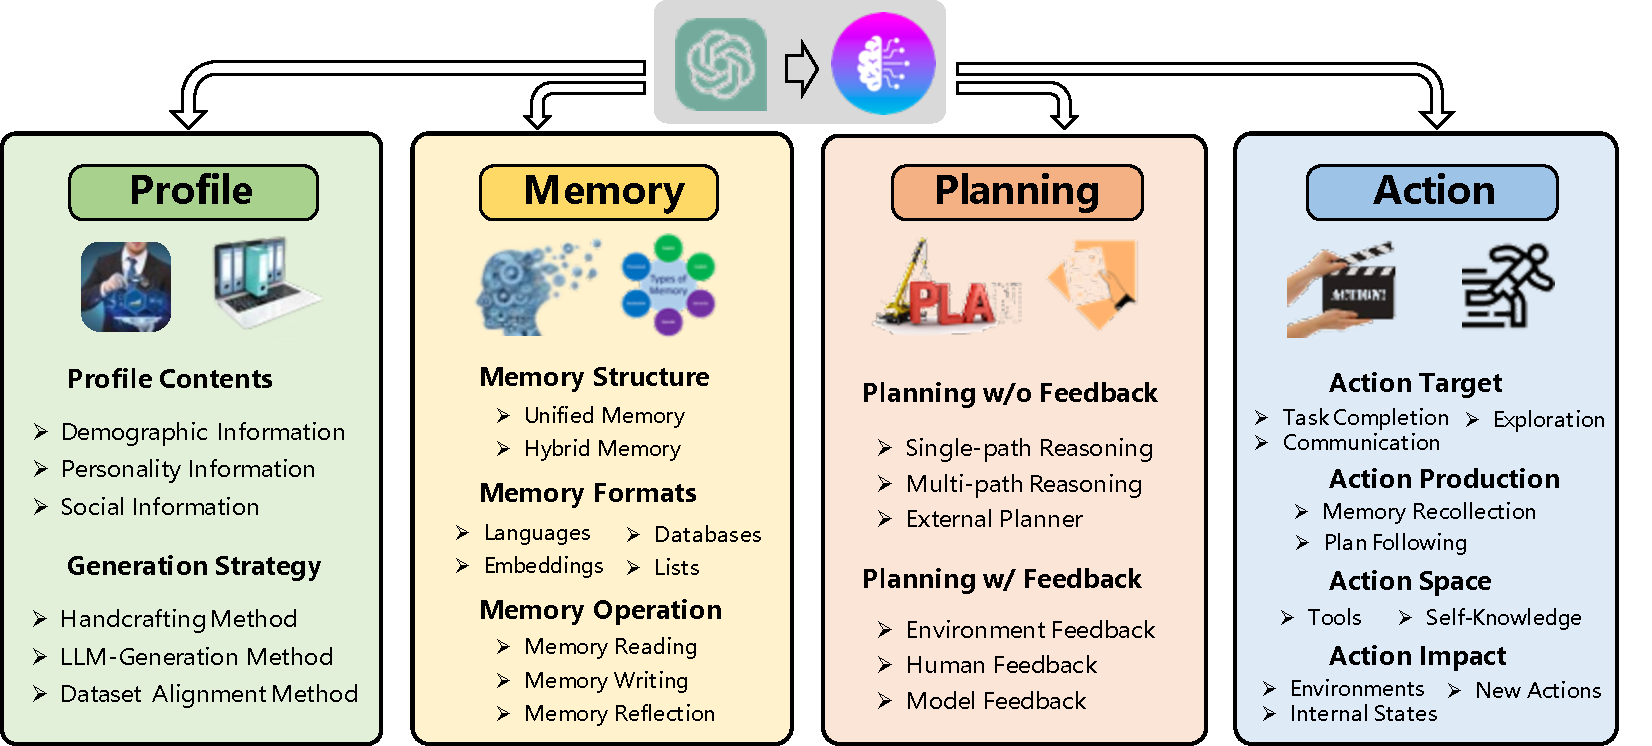
\includegraphics[width=1\textwidth]{Figures/agent_four_modules.pdf}
    \caption{A general framework to reason about LLM-based agents.}
    \label{fig: agent}
\end{figure}

An LLM-based agent example is detailed and explained in Section \ref{sec:myagent}.

\subsection{Scaffolded LLMs: a way towards AGI?}
The pursuit of Artificial General Intelligence (AGI) has long been a goal in the field of machine learning and artificial intelligence. While current advancements have resulted in powerful systems capable of achieving superhuman performance on specialized tasks, the emergence of AGI remains elusive. In this section, we explore whether the current machine learning paradigm—particularly through the scaling of models, data, and computational power—can ultimately achieve AGI or whether inherent limitations prevent this.

Let's first roughly define what we mean with AGI.
\begin{definition}[Artificial General Intelligence]
    An Artificial General Intelligence is a program that can adapt and act (through tools or actuators), with effectiveness, to an unseen environment to reach (maximize) a planned goal autonomously.
\end{definition}

Some comments on the definition:
\begin{itemize}
    \item \textbf{Tools and actuators} refer to everything that is not the 'brain' itself but is necessary for decision-making or action: hardware, sensors, robotic arms, other software (e.g., symbolic systems), databases, external structured knowledge, etc.
    \item \textbf{The environment} is the world in which the AGI is deployed, where it begins to observe, plan, and act autonomously. This can be a fully virtual world, a physical world, or a hybrid. \footnote{There is a concern in the research community that containing AGI purely within a virtual environment may be unsafe if the AGI develops inner goals or self-consciousness.}
    \item \textbf{Effectiveness} should be measurable by the increase of productivity in tasks that hold meaning for human purposes.
\end{itemize}

We can divide an AGI into four logical modules\footnote{A different formalization may better suit based on specific contexts.}: 
\begin{itemize}
    \item \textbf{Planning:} The ability to develop a sequence of steps toward achieving a goal. For AGI to be effective, planning must adapt to environmental feedback and leverage available tools.
    \item \textbf{Reasoning:} The ability to decide how to execute planned steps effectively. This involves problem-solving and decision-making based on both internal knowledge and external stimuli.
    \item \textbf{Memory:} The capacity to store, update, and retrieve information. Memory aids the AGI in planning and reasoning by providing historical context and learned knowledge.
    \item \textbf{Action:} The capability to execute decisions, translating plans and reasoning into tangible outcomes. Action is the interface between the AGI's internal reasoning and the environment.
\end{itemize}
We notice that the above characteristics are deeply interconnected: planning, reasoning and memory are distinct but indissoluble abilities.

We can be convinced that no further characteristics are strictly needed by analysing the previous modules. However, sometimes further elements are considered; most of them are just ways to realize one of the above modules:
\begin{itemize}
    \item \textbf{Self-consciousness:} While often associated with human intelligence, it is not necessarily a requirement for a program to disruptively impact our society with general-purpose abilities.
    \item \textbf{Reinforcement learning to set a goal:} Goal-setting can be achieved through other paradigms (like scaffolding techniques).
    \item \textbf{Symbolic reasoning:} Symbolic systems can be externalized and accessed when necessary, rather than being an intrinsic component of the AGI core.
\end{itemize}

\paragraph{How Can Intelligence Emerge?}
One key question is whether the current paradigm, centred around prediction tasks, can lead to the emergence of true reasoning and intelligence. The next-token prediction task, as seen in large language models (LLMs), enables these systems to generate coherent, contextually accurate responses. However, while this form of predictive learning has led to impressive advancements in natural language understanding and generation, there remains doubt about whether it can scale to AGI. 

Reasoning may require a more complex set of interactions than simple prediction. While predictive models exhibit "emergent" capabilities as they scale, it is unclear whether these emergent properties can replicate the generality, flexibility, and autonomy of human reasoning.

As models grow in size and access more diverse data, there may be exponential improvements in performance on a wide range of tasks. We can refer to the past, somehow available, knowledge or experience as culture: the broader the knowledge base a system can draw from, the more it can mimic human-like general intelligence. An AGI capable of understanding and integrating diverse cultural elements, even with poor reasoning capabilities, may show a form of intelligence explosion as it adapts to new contexts and generates novel solutions. Some forms of external symbolic reasoning tools are good examples of cultural exploitation.

\paragraph{Can Scaffolding Transform Reasoning into AGI?}
Scaffolding refers to the external structures or support systems that enhance the model's ability to perform complex tasks by interacting with environments, tools, or knowledge sources outside of the core model itself. These scaffolds can provide the LLM with additional capabilities that it may not inherently possess, allowing it to extend its reasoning, decision-making, and action-execution abilities.

Key elements of scaffolding in LLM-based agents include:
\begin{itemize}
\item External tools: APIs, symbolic reasoning systems, calculators, or databases that the LLM can query to augment its capabilities.
\item Environmental feedback: Continuous interaction with the external world where the agent receives feedback, enabling iterative improvement or course correction.
\item Task-specific frameworks: Predefined structures or protocols that guide the LLM in solving problems or completing tasks more effectively, such as step-by-step instructions.
\end{itemize}

In human cognitive development, scaffolding is provided by social and environmental inputs. For AGI, scaffolding could take the form of external tools (e.g., databases, reasoning engines, symbolic systems) or frameworks that allow the system to extend its capabilities beyond its core architecture.

The idea is that by embedding an AI in a scaffolded system, it could exhibit forms of reasoning that would otherwise be difficult or impossible in a standalone, unsupervised learning environment. 

In conclusion, while scaling the current machine learning paradigm leads to emergent capabilities, it remains uncertain (but possible) whether this alone can achieve AGI.


\section{Evaluating LLMs: best practices}
\label{sec:evaluatingllm}
Evaluations refer to a broad category of approaches that are generally oriented towards a systematic measurement of properties in AI systems.
More concretely, evaluations typically attempt to make a quantitative or qualitative statement about the capabilities or propensities of a machine learning model. 

Evaluations can be subdivided into two, often overlapping, categories:
\begin{itemize}
    \item Benchmarking: is a standard or set of standards used to measure and compare the performance of various systems, processes, or components. In evaluating LLMs, benchmarks are specific datasets and associated metrics used to assess and compare the capabilities of different models in a reproducible way.
    
    \item Red-Teaming: is a process used to challenge and improve the robustness, security, and ethical countermeasures of a system by adopting an adversarial approach. In the context of LLMs, red-teaming involves simulating attacks or adversarial inputs to identify vulnerabilities, biases or dangerous behaviours.
\end{itemize}

Since evaluations often aim to estimate an upper bound of capabilities, it is important to understand how to elicit maximal, rather than average, capabilities. Different improvements to prompt engineering have continuously raised the bar and thus made it hard to estimate whether any particular negative/positive result is meaningful or whether a better technique could invalidate it. Furthermore, small rephrasing and changes in the input prompts may result in performance changes to volatile evaluations. A partial solution is to build a set of similar prompts and aggregate in a canonical way the performances (for example by averaging).

LLM evaluation is a burgeoning field, with no universally accepted standards established yet. Despite this, we can identify several important properties that an ideal benchmark for evaluating LLMs should possess:

\begin{itemize}
    \item \textbf{Future-proof}: The benchmark should maintain a consistent level of difficulty, even as further research advances or new tools are developed. It needs to be challenging enough to evaluate future models effectively. This ensures that the benchmark remains relevant and provides meaningful insights into model performance over time.
    
    \item \textbf{Resistant to Prior Knowledge}: Programmers should not be able to gain an unfair advantage by having prior knowledge of the benchmark. For instance, we should avoid using datasets that are readily available on the web, as familiarity with these datasets could skew the evaluation results. A solution is to maintain locally most of the benchmarks (shared only by request).
    
    \item \textbf{Consistent}: The results obtained from the benchmark should be reliable and reproducible. This means that repeated runs of the evaluation under the same conditions should yield roughly the same results. Consistency is crucial for comparing different models and ensuring that the evaluation process is fair and unbiased.
    
    \item \textbf{Intrinsic Difficulty}: The benchmark's difficulty should arise from the inherent complexity of the tasks it comprises, rather than from extraneous factors or overly structured tasks. This ensures that the evaluation focuses on the model's capabilities and understanding while avoiding insignificant bottlenecks.
    
    \item \textbf{Automatic Real-Valued Scoring}: The benchmark should include a mechanism for automatic scoring that yields real-valued results. This allows for precise and quantitative assessment of model performance, facilitating clear comparisons and analysis. Automatic scoring also reduces the potential for human error or subjectivity in the evaluation process.
    
    \item \textbf{Meaningful Tasks}: The tasks included in the benchmark should be meaningful and relevant to real-world applications. This ensures that the evaluation provides valuable insights into how well the models can perform tasks that are of practical importance. Meaningful tasks also help to ensure that improvements in benchmark performance translate to genuine advancements in the model's utility and effectiveness in real-world scenarios.
\end{itemize}

By adhering to these properties, an ideal benchmark can provide a robust, reliable, and meaningful assessment of LLM performance. However, since standards are not yet refined and the capabilities are sensitive to the agent design choices (which can be adapted to each LLM) a flawless and objective evaluation cannot be achieved.

Our project aims to develop a benchmark to assess the potential of current LLM-based agents (with the best prompts and tools we managed to develop or adapt from literature) to analyze security protocols with a formal prover (Tamarin). 